\chapter{Calcolo differenziale}
\pagestyle{plain}
\thispagestyle{empty}
\pagestyle{fancy}
In questo capitolo andremo a generalizzare il concetto di derivata  alle funzioni vettoriali (sia nell'insieme di definizione che nell'insieme di arrivo). Tutto ciò avverrà passando, naturalmente, per la definizione di funzione differenziabile e, successivamente, andando ad enunciare i teoremi riguardo all'esistenza e l'unicità del differenziale, soffermandosi in particolare modo nell'individuare delle espressioni per il differenziale, il gradiente e la matrice jacobiana e, per poi passare, alle derivate seconde, necessarie per lo studio dei massimi e dei minimi tramite lo studio della matrice hessiana. 

\section{Funzione differenziabile}

\begin{definition}[funzione differenziabile in un punto e matrice jacobiana]
Sia $\Omega \subseteq \mathbb{R}^n$ aperto e $x_0 \in \Omega$. Diremo che $f: \Omega \to \mathbb{R}^m$ è differenziabile in $x_0$ se $\exists L: \mathbb{R}^n \to \mathbb{R}^m$ lineare tale che
$$
\frac{f(x_0 + h)-f(x) - L(h)}{|h|} \stackrel{h \to 0}{\to} 0
$$
dove l'applicazione $L = df(x_0): \mathbb{R}^n \to \mathbb{R}^m$ è detto il differenziale di $f$ in $x_0$. La matrice $Df(x_0) \in \mathbb{R}^{m \times n}$ che rappresenta $df(x_0)$ rispetto alla base canonica è detta \textbf{matrice jacobiana} di $f$ in $x_0$.
\end{definition}

\begin{figure}[htbp]
\centering
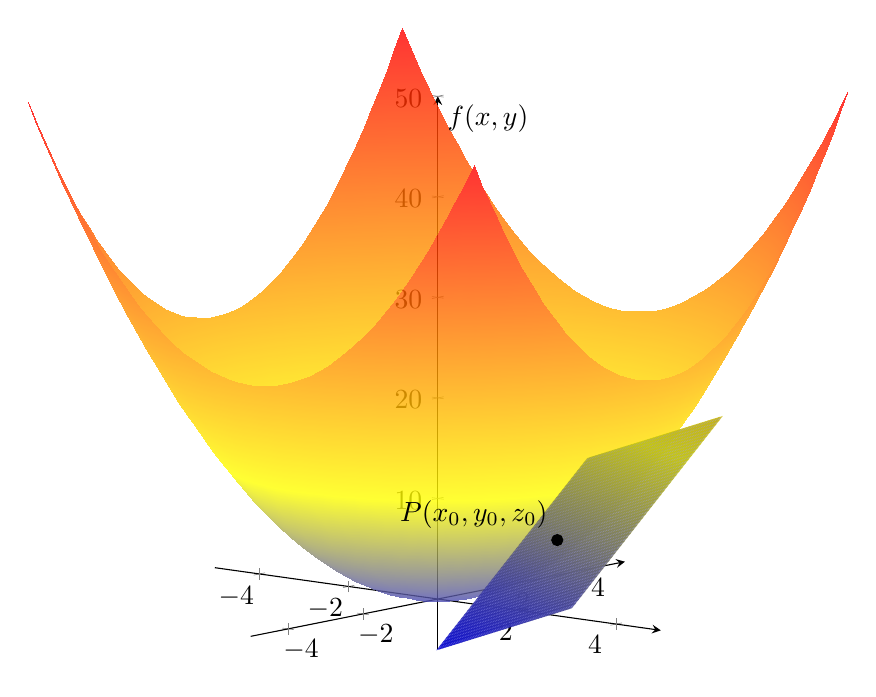
\begin{tikzpicture}
    % Definisco lo stile dei vettori
    \tikzset{vector/.style={-stealth, thick, color=black}}

    % Parametri per il punto di contatto
    \def\xo{1}
    \def\yo{2}
    \def\zo{5} % Calcola z0 = f(x0, y0)

    % Derivate parziali della funzione f(x, y) = x^2 + y^2 nel punto (x0, y0)
    \def\fx{2*\xo} % = 2
    \def\fy{2*\yo} % = 4

    % Disegno la superficie
    \begin{axis}[
        width=12cm,
        view={40}{10}, % Angolazione impostata
        axis lines=middle,
        zlabel={$f(x,y)$},
        clip=false,
        domain=-5:5,
        y domain=-5:5,
        samples=50,
        z buffer=sort
    ]

    % Grafico della superficie con colore visibile
    \addplot3[surf, opacity=0.8, shader=interp]
        {x^2 + y^2}; % Superficie f(x, y) = x^2 + y^2

    % Disegno del piano tangente al punto (x0, y0)
    \addplot3[surf, opacity=0.7, fill=blue!50, domain=0:3, y domain=0:4]
        {(\zo + \fx*(x - \xo) + \fy*(y - \yo))}; % Piano tangente

    % Punto di contatto sulla superficie
    \addplot3[mark=*, mark options={color=black}, only marks] coordinates {(\xo,\yo,\zo)};
    \node at (axis cs: \xo,\yo,\zo+0.2) [anchor=south east] {$P(x_0, y_0, z_0)$};
    \end{axis}
\end{tikzpicture}
\caption{Nozione di differenziabilità da un punto di vista geometrico: la funzione $x^2 + y^2$ è differenziabile nel punto $x_0=(1, 2, 5)$ e, dunque, possiamo approssimare la funzione in un intorno di $x_0$ alla funzione alla funzione lineare $L$ tale che $L(x, y) = 5 + 2(x-1) + 4(y-2)$}
\end{figure}
\begin{remark}
Naturalmente diremo che $f$ è differenziabile in $\Omega$ se è differenziabile $\forall x \in \Omega$.
\end{remark}
\noindent Come avevo anticipato alla fine dello scorso capitolo, possiamo rendere molto semplice la trattazione del calcolo differenziabile tramite i simboli di Landau. Mostriamo per esempio la seguente proposizione:
\begin{prop}
$f: \Omega \to \mathbb{R}^m$ con $\Omega \subseteq \mathbb{R}^n$ aperto. Diremo che $f$ è differenziabile in $x_0 \in \Omega \iff \exists L:\mathbb{R}^n \to \mathbb{R}^m$ lineare tale che $f(x_0 + h) = f(x_0) + L(h) + o(h)$ per $h \to 0 \iff $(cambio di variabile) $\exists L: \mathbb{R}^n \to \mathbb{R}^m$ lineare tale che $f(x) = f(x_0) + L(x-x_0) + o(x-x_0)$ per $x \to x_0$.
\end{prop}
\begin{proof}
Se $f$ è differenziabile in $x_0 \in \Omega$, sappiamo che $\exists L : \mathbb{R}^n \to \mathbb{R}^m$ tale che
$$
\frac{f(x_0 + h) - f(x_0) - L(h)}{|h|} \to 0 \implies f(x_0 + h) - f(x_0) - L(h) = o(|h|) \text{ per } h \to 0
$$
che è equivalente (per cambiamento di variabile) a:
$$
f(x) = f(x_0) + L(x-x_0) + o(|x-x_0|) \text{ per } x \to x_0
$$
Il viceversa è analogo, siccome se
\begin{align*}
&f(x_0 + h) - f(x_0) - L(h) = o(|h|) \implies \frac{f(x_0 + h) - f(x_0) - L(h)}{|h|} \to 0 \implies \\
&\text{f è differenziabile in } x_0
\end{align*}
\end{proof}
\noindent Ma in sostanza che cosa vuol dire essere differenziabili? Come forse alcuni avranno potuto capire dalla definizione, essere differenziabili vuol dire che è possibile approssimare la funzione, in quel punto $x_0 \in \Omega$ in cui è differenziabile, ad una applicazione affine del tipo $$a(x) = f(x_0) + df(x_0)(x-x_0)$$ che sarebbe, in maniera impropria, ciò che, in gergo da fisici, diciamo essere un'approssimazione del primo ordine. \\
Dopo questa definizione siamo persino pronti a definire il concetto di derivata direzionale, nozione strettamente connessa a quella di differenziabilità.
\begin{definition}[derivata direzionale]
Sia $\Omega \subseteq \mathbb{R}^n$ aperto, $x_0 \in \Omega$, $f: \Omega \to \mathbb{R}$ e sia $v \in \mathbb{R}^n \setminus \{ \underline{0} \}$. Definiamo la derivata direzionale rispetto a $v$ il limite (se esiste!)
$$
\partial_v f(x_0) = \lim_{t \to 0} \frac{f(x_0 + tv) - f(x_0)}{t}
$$
\end{definition}
\noindent Nel caso in cui $v = e_i$ la derivata direzionale è detta derivata parziale rispetto a $x_i$.
\begin{remark}
La derivata parziale rispetto a $x_i$ è, di fatto, la derivata di una funzione di una sola variabile. Pertanto queste posso essere svolte tenendo "costanti" le altre variabili $x_j$ con $j \neq i$ e calcolare la derivata come usualmente si faceva ad Analisi 1
\end{remark}
\noindent Ricollegandoci all'osservazione fatta qua sopra, infatti, possiamo osservare che:
$$
\partial_{e_1} f(x_0) = \lim_{t \to 0} \frac{f(x_0 + te_1) - f(x_0)}{t} = \lim_{t \to 0} \frac{f(x_1 + t, x_2, \ldots) - f(x_1, x_2, \ldots )}{t}
$$
Siamo adesso pronti ad enunciare il seguente risultato, che ci dà qualche informazione su come sia il differenziale:
\begin{theorem}[DF1]
Se $f: \Omega \to \mathbb{R}$ è differenziabile in $x_0$ allora $\exists \partial_v f \, \forall v \in \mathbb{R}^n \setminus \{ \underline{0} \}$ e vale che
$$
df(x_0)(v) = \partial_v f(x_0)
$$
\label{thm:teorema_df1}
\end{theorem}
\begin{proof}
Siccome $f$ è differenziabile in $x_0 \in \Omega$ allora $\exists L: \mathbb{R}^n \to \mathbb{R}$ tale che $f(x_0 + tv) = f(x_0) + L(tv) + o(|tv|)$ dove $|tv| \to 0$ per $v \in \mathbb{R}^n \setminus \{ \underline{0} \}$. Ma questo allora implica che
\begin{align*}
&\frac{f(x_0 + tv) - f(x_0) - L(|tv|)}{t} \to 0 \implies \frac{f(x_0 + tv) - f(x_0) - tL(v)}{t} \to 0 \implies \\ &\implies \lim_{t \to 0} (\frac{f(x_0 + tv) - f(x_0)}{t} - L(v)) \to 0 \implies \implies \exists \partial_v f(x_0) = L(v) = df(x_0)(v)
\end{align*}
\end{proof}
\begin{theorem}[rappresentazione e unicità del differenziale]
Se $f: \Omega \to \mathbb{R}$ è differenziabile in $x_0 \in \Omega$  allora il differenziabile di $f$ nel punto $x_0 \in \Omega$ è unico e
$$
df(x_0)(\xi_1, \ldots \xi_n) = \sum_{j=1}^n \xi_j \frac{\partial f}{\partial x_j}(x_0)
$$
\end{theorem}
\begin{proof}
Preso $v \in \mathbb{R}^n \setminus \{ \underline{0} \}$, allora 
$$
v = \sum \xi_i e_i \simeq (\xi_1, \ldots, \xi_n) \implies df(x_0)(v) = \sum_{j = 1}^n \xi_j df(x_0)(e_j) = \sum_{j=1}^n \xi_j \partial_{e_j} f(x_0)
$$
dove abbiamo solamente sfruttato la linearità della funzione differenziabile e il fatto che $df(x_0)(e_j) = \frac{\partial f}{\partial x_j}(x_0)$. L'unicità del differenziabile deriva dal fatto che se supponiamo per assurdo che esista $L' \neq df(x_0)$ lineare, tali che $L(v) = df(x_0)(v) \, \forall v \in \mathbb{R}^n \setminus \{ \underline{0} \}$ allora preso un $v \in \mathbb{R}^n \setminus \{ \underline{0} \}$ avremo che:
$$
L(v) = \sum_j^n \xi_j L(e_j) = \sum_j^n \xi_j df(x_0)(e_j) = df(x_0)(v)
$$
dove tutte queste uguaglianze sono ottenute sfruttando la linearità di $L$ e $df(x_0)$. L'unica possibilità (siccome questa è una relazione valida per ogni vettore) è che $L(e_j) = df(x_0)(e_j) \, \forall j$ ma allora queste due applicazioni lineari coincidono, giungendo ad un assurdo. Quindi il differenziale $df(x_0)$ è unico.
\end{proof}
\noindent Possiamo dunque definire il concetto di gradiente:
\begin{definition}[gradiente di una funzione]
Sia $f: \Omega \to \mathbb{R}$ con $\Omega \subseteq \mathbb{R}^n$, $x_0 \in \Omega$ e $f$ differenziabile in $x_0$. Allora definiamo il gradiente $$\nabla{f(x_0)} = \left( \frac{\partial f}{\partial x_1}(x_0), \ldots, \frac{\partial f}{\partial x_n}(x_0) \right) = \sum_{i=1}^n \frac{\partial f}{\partial x_i}f(x_0)e_i \in \mathbb{R}^n$$
\end{definition}
\begin{remark}
Il gradiente di $f$ nel punto $x_0$ è di fatto il vettore che ha come componenti le derivate parziali di $f$
\end{remark}
\noindent Dalla formula precedente è possibile ricavare che
$$
df(x_0)(v) = \innerprod{\nabla{f(x_0)}}{v}
$$
\begin{remark}
Da qua possiamo vedere il grandissimo problema di definire il gradiente: per definire le derivate parziali, di fatto, abbiamo solamente fatto riferimento alla natura da "spazio metrico" di $\mathbb{R}^n$, quindi in generale potremmo andare a definire la derivata su una classe maggiore di insiemi rispetto che a $\mathbb{R}$ e $\mathbb{C}$. Per definire il gradiente, però, abbiamo richiesto il prodotto scalare, che è una condizione decisamente più forte che alla semplice distanza.
\end{remark}
\noindent Cerchiamo adesso di capire che cosa rappresenta il gradiente. Il gradiente possiamo vederlo come la direzione in cui la funzione ha la massima pendenza\footnote{questo è particolarmente comodo, per gli algoritmi locali di minimizzazione o massimizzazione, in cui si sfrutta la pendenza della funzione nel punto per trovare i massimi e i minimi locali.}. Per vedere questo possiamo considerare il vettore $v = \frac{\nabla f(x_0)}{|\nabla f(x_0)|}$ e considerando il vettore $w \in \mathbb{R}^n$ tale che $|w| = 1$ allora
$$
\partial_w f(x_0) = \innerprod{\nabla{f(x_0)}}{w} \leq |\nabla{f(x_0)}| \, |w| = |\nabla{f(x_0)}|
$$
per la disuguaglianza di Cauchy-Schwarz. Tuttavia si osserva che
$$
|\nabla{f(x_0)}| = \innerprod{\nabla{f(x_0)}}{v} = \innerprod{\nabla{f(x_0)}}{\nabla{f(x_0)}} \frac{1}{|\nabla{f(x_0)}|} = \partial_v f(x_0)
$$
dunque
$$
\partial_w f(x_0) \leq \partial_v f(x_0)
$$
Per poter ampliare la nostra teoria ed esprimere correttamente il differenziale è necessario riprendere la definizione di spazio duale dal corso di Geometria:
\begin{definition}[spazio duale]
Sia $V$ uno spazio vettoriale sul campo $\mathbb{K}$, definiamo lo spazio duale $V^{*}$ come lo spazio vettoriale dei funzionali lineari $f: V \to \mathbb{K}$. In simboli
$$
V^{*} = \{f \, | \, f: V \to \mathbb{K} \}
$$
\end{definition}
\noindent Introduciamo, a questo punto, le funzioni proiezioni $\pi_i: \mathbb{R}^n \to \mathbb{R}$ tali che $x = (x_1, \ldots, x_n) \mapsto x_i$, ovvero le funzioni che associano l'$i$-esima componente del vettore $x \in \mathbb{R}^n$. \\
Osserviamo naturalmente che
$$
|\pi_i(x)| = |x_i| \leq |x| \, \forall x \in \mathbb{R}^n
$$ 
e notiamo che le funzioni proiezioni sono lineari e se $L: \mathbb{R}^n \to \mathbb{R}$ è lineare, allora
$$
L(x) = L \left( \sum_{i=1}^n x_i e_i \right) = \sum_{i=1}^n x_i L(e_i) = \sum_{i=1}^n \pi_i(x) L(e_i)
$$
e, naturalmente, per come è definita $L$ abbiamo che $L(e_i) = a_i \, \forall i$, quindi ogni funzione lineare da $\mathbb{R}^n$ a $\mathbb{R}$ è una combinazione lineare delle funzioni lineari $\pi_i$. \\
Passando in $\mathbb{R}^n$, osserviamo che queste funzioni proiezioni sono una base dello spazio duale $(\mathbb{R}^n)^{*}$ e definiamo $dx_i = \pi_i$. \\
\begin{prop}
Sia $f: \Omega \to \mathbb{R}, f$ differenziabile in $x_0 \in \Omega$. Allora
$$
df(x_0) = \sum_{i=1}^n \partial_{x_i} f(x_0)dx_i = \partial_{x_1} f(x_0)dx_1 + \ldots + \partial_{x_n} f(x_0)dx_n \in (\mathbb{R}^n)^{*}
$$
\end{prop}
\begin{proof}
Dato $v=(\xi_1, \ldots \xi_n) = \sum_{i=1}^n \xi_i e_i$ allora
$$
df(x_0)(v) \stackrel{\text{per linearità}}{=} \sum_{i=1}^n \xi_i df(x_0)(e_i) = \sum_{i=1}^n \pi_i(v) df(x_0)(e_i)$$
dove l'ultima uguaglianza si è ottenuta osservando che $\xi_i = \pi_i(v) = dx_j(v)$. A questo punto, ricordando che $df(x_0)(e_i) = \partial_{x_i} f(x_0)$ in virtù del teorema~\ref{thm:teorema_df1}, otteniamo la tesi, siccome
$$\sum_{i=1}^n \partial_{x_i} f(x_0) dx_i(v) \implies df(x_0) = \sum_{i=1}^n \partial_{x_i} f(x_0) dx_i
$$
\end{proof}
\begin{remark}
Data $f: \Omega \to \mathbb{R}$, possiamo allora vedere il differenziale come una funzione che ad ogni punto $p \in \Omega$ associa $df(p) \in (\mathbb{R}^n)^{*}$, ovvero $df: \Omega \mapsto (\mathbb{R}^n)^{*}$
$$
df(p) = \sum_{i=1}^n df(p)dx_i \, \forall p \in \Omega
$$
\end{remark}
Alla luce dell'osservazione qua sopra possiamo dunque dare la seguente definizione:
\begin{definition}[1-forma differenziale]
Diremo che $\omega: \Omega \to (\mathbb{R}^n)^{*}$ con $\Omega \subseteq \mathbb{R}^n$ aperto è una $1$-forma differenziale su $\Omega$. Inoltre, $\forall p \in \Omega$ avremo un'unica $n$-upla di coefficiente $(a_1(p), \ldots a_n(p))$ dipendenti da $p$ tali che
$$
\omega(x) = \sum_{i=1}^n a_i(x)dx_i
$$
\end{definition}
\begin{remark}
\noindent Quando abbiamo a che fare con $\omega$ $1$-forma differenziale possiamo andare a definrie delle funzioni $a_1(x), \ldots a_n(x): \Omega \to \mathbb{R}$ tali che
$$
\omega(x) = \sum_{j=0}^n a_j(x)dx_j
$$
\end{remark}
\begin{definition}[campo vettoriale]
Sia $\Omega \subseteq \mathbb{R}^n$ aperto, diremo che $F$ è un campo vettoriale se $F: \Omega \to \mathbb{R}^n$, ovvero $F(p) = \sum\limits_{j=1}^n f_j(p)e_j = (f_1(p), \ldots f_n(p))$ ove $f_j: \Omega \to \mathbb{R}$ sono le componenti di $F$
\end{definition}
\begin{remark}
Se $\omega: \Omega \to (\mathbb{R}^n)^{*}$ è una 1-forma differenziale e $F: \Omega \to \mathbb{R}^n$ è un campo vettoriale, allora $\innerprod{\omega}{F}: \Omega \to \mathbb{R}$ tale che $p \mapsto \omega(p)F(p)$ è uno scalare, ovvero è indipendente dal fatto che utilizziamo le basi canoniche per rappresentare $\omega$ e $F$. In questo caso diremo che la 1-forma differenziale $\omega$ si è contratta su $F$
\end{remark}
Enunciamo adesso il risultato più importante di questo capitolo:
\begin{theorem}
Sia $\Omega \subseteq \mathbb{R}^n$ aperto, $p_0 \in \Omega$ e sia $f: \Omega \to \mathbb{R}^m$ ($\iff f=(f_1, \ldots f_m)$ con $f_j: \Omega \to \mathbb{R} \, \forall j$). Allora 
$$
f \text{ è differenziabile in } p_0 \iff \text{ogni componente di } f_j \text{ è differenziabile in } p_0
$$
In ogni caso avremo che
$$
D(f(x_0)) = \begin{pmatrix}
\nabla{f_1(p_0)} \\
\nabla{f_2(p_0)} \\
\vdots \\
\nabla{f_m(p_0)} \\
\end{pmatrix} \in \mathbb{R}^{m \times n}
$$
\end{theorem}
\begin{proof} \hspace{1em} \\
$\boxed{\Rightarrow}$: se $f$ è differenziabile allora possiamo definire la funzione $\pi_i \circ df(p_0): \mathbb{R}^n \to \mathbb{R}$ e sappiamo che
\begin{equation}
f(x) = f(p_0) + df(p_0)(x-p_0) + o(x-p_0) 
\label{eq:appl_aff}
\end{equation}
e osserviamo, ricordando che $x_i \leq |x|$ con dove $x_i$ rappresenta l'$i$-esima, che
\begin{align*}
&\frac{|\pi_i \circ o(x-p_0)|}{|x-p_0|} \leq \frac{|o(x-p_0)|}{|x-p_0|} \to 0 \\
&\implies \pi_i \circ o(x-p_0) = o(x-p_0)
\end{align*}
dove l'ultima affermazione segue, banalmente, dal teorema del confronto. \\
Componendo $\pi_i$ all'applicazione lineare affine otteniamo che
$$
\pi_i \circ f(x) = f_i(p_0) + (df(p_0))_i (x-p_0) + o(x-p_0) \, \text{per } x \to p_0 
$$
Per l'unicità del differenziale di $f_i$ (che ricordiamo essere una funzione $\Omega \to \mathbb{R}$, dunque sappiamo, per il teorema precedente, che il suo differenziale è unico) segue che
$$
\pi_i \circ L(x) = df_i(p_0)(x) = \innerprod{\nabla{f(p_0)}}{x}
$$
il che naturalmente implica che
\begin{align*}
&L(x) = \sum_{i=1}^m L_i(x) e_i = \sum_{i=1}^m (\pi_i \circ L)(x) e_i = \sum_{i=1}^m \innerprod{\nabla{f_i(x_0)}}{x} e_i = \begin{pmatrix} \partial_{x_1} f_1(p_0) & \ldots & \partial_{x_n} f_1(p_0) \\
\vdots & \vdots & \vdots \\
\partial_{x_1} f_m(p_0) & \ldots & \partial_{x_n} f_m(p_0)  \end{pmatrix} \begin{pmatrix}
x_1 \\
x_2 \\
\vdots \\
x_n
\end{pmatrix} = \\
&= Df(x_0)x
\end{align*}
e questo mostra la tesi. \\
$\boxed{\Leftarrow}$: se $f_i$ è differenziabile in $p_0 \, \forall i \in 1, \ldots, n$ definiamo $df_i(x_0): \mathbb{R}^n \to \mathbb{R}$ e osserviamo che
\begin{align*}
&f(p_0 + h) - f(p_0) = \sum_{i=1}^m (f_i(p_0 + h) - f_i(p_0))e_i = \sum_{i=1}^m (df_i(p_0)(h) + o(h))e_i = \\
&= \sum_{i=1}^m df_i(p_0)(h)e_i + \sum_{i=1}^m o_i(h)e_i = L(h) + o(h) \implies f \text{ è differenziale in } p_0
\end{align*}
dove, naturalmente, abbiamo che
$$
L(h) = \sum_{i=1}^m \innerprod{\nabla{f(p_0)}}{h}e_i = Df(x_0)h
$$
Abbiamo dunque ottenuto la tesi.
\end{proof}
\begin{cor}
Il teorema precedente mostra anche come il differenziale sia unico anche nel caso di funzioni vettoriali.
\end{cor}
\begin{theorem}[del differenziale totale]
Sia $f: \Omega \to \mathbb{R}, \Omega \subseteq \mathbb{R}^n$ aperto e $p_0 \in \Omega$. Se $$\exists \partial_{x_j} f: B(p_0, r) \to \mathbb{R} \, \forall j \in \{1, \ldots n\} \text{ con } B(p_0, r) \subseteq \Omega$$ e se 
$$
\partial_{x_j} f \text{ sono tutte continue in } p_0 \, \forall j \in \{1, \ldots, n \}$$ allora $f$ è differenziale in $p_0$
\end{theorem}
\begin{proof}
Consideriamo $h=\sum\limits_{j=1}^n h_j e_j = (h_1, \ldots h_n)$. Osserviamo che posto
$$
L(h) = \sum_{j=1}^n \partial_j f(p_0)h_j
$$
possiamo notare come
\begin{align*}
&f(p_0 + h) - f(p_0) - L(h) = \\
&= f(p_0 + h) - f \left( p_0 + \sum_{i=1}^{n-1} h_j e_j \right) + f \left( p_0 + \sum_{i=1}^{n-1} h_j e_j \right) - f \left( p_0 + \sum_{i=1}^{n-2} h_j e_j \right) + f \left( p_0 + \sum_{i=1}^{n-2} h_j e_j \right) - \ldots \\ 
&- f(p_0) - L(h)
\end{align*}
possiamo raggruppare a 2 a due i termini, notando che:
\begin{align*}
&\left( f(p_0 + h) - f(p_0 + \sum_{i=1}^{n-1} h_j e_j) \right) + \left( f(p_0 + \sum_{i=1}^{n-1} h_j e_j) - f(p_0 + \sum_{i=1}^{n-2} h_j e_j) \right) + \ldots + \\
&\left( f(p_0 + h_1) - f(p_0) \right) - L(h)
\end{align*}
al raggruppamento $j$-esimo teniamo fisso la $n-j+1$ componente dell'argomento della funzione sulla sinistra, pertanto possiamo applicare il teorema di Lagrange se definiamo una funzione dipendente esclusivamente dalla variabile $h_j$, dunque:
\begin{align*}
    & f(p_0 + h) - f(p_0) - L(h) = \\
    & = \quad \partial_{x_n} f (p_0 + \sum_{j=1}^{n-1} h_j e_j + \theta_n h_n e_n) h_n + \partial_{x_{n-1}} f(p_0 + \sum_{j=1}^{n-2} h_j e_j + \theta_{n-1} h_{n-1} e_{n-1}) h_{n-1} + \ldots - L(h) = \\
    & = \quad \left(\partial_{x_n} f(p_0 + \sum_{j=1}^{n-1} h_j e_j + \theta_n h_n e_n) - \partial_{x_n} f(p_0)\right) h_n + \left(\partial_{x_{n-1}} f(p_0 + \sum_{j=1}^{n-2} h_j e_j + \theta_{n-1} h_{n-1} e_{n-1}) - \right. \\
    & -\partial_{x_{n-1}} f(p_0) \bigg) h_{n-1} + \ldots = o(1) h_n + o(1) h_{n-1} + \ldots + o(1) h_1 \quad \text{per } |h| \to 0.
\end{align*}
dove la penultima uguaglianza segue da come avevamo definito $L(h)$ e l'ultima dalla continuità delle derivate parziali che avevamo richiesto nelle ipotesi. Dunque, per $|h| \to 0$, osserviamo che $o(1)h_j \leq o(1)|h| \implies \frac{o(1)h_j}{|h|} \leq \frac{o(1)|h|}{|h|} = o(1) \implies o(1)h_j = o(h)$ e chiaramente $\frac{o(1)h_n + \ldots + o(1)h_1}{|h|} \to 0$. Dunque 
$$
f(p_0 + h) - f(p_0) - L(h) = o(h)
$$
ovvero la tesi.
\end{proof}
Prima di procedere con la prossima dimostrazione, introduciamo la norma di Hilbert-Schmidt
\begin{definition}[norma di Hilbert-Schmidt]
Sia $A \in \mathbb{R}^{m \times n}$, definiamo
$$
|| A || = \sqrt{\sum a_{ij}^2} \text{ è la norma di Hilbert-Schmidt}
$$
\end{definition}
\begin{remark}
$|Lx| \leq ||A|| \, |x| \, \, \forall x \in \mathbb{R}^n$
\end{remark}
\begin{theorem}[differenziale della composizione]
Sia $f: \Omega \to \mathbb{R}^m, g: U \to \mathbb{R}^k$ con $\Omega \subseteq \mathbb{R}^n$ aperto, $U \subseteq \mathbb{R}^m$ aperto, $f(\Omega) \subseteq U$ e sia $p_0 \in \Omega$. Allora se $f$ differenziabile in $p_0$ e $g$ differenziabile in $f(p_0)$ allora
$$
g \circ f: \Omega \to \mathbb{R}^k \text{ è differenziabile in } p_0
$$
Inoltre, in tal caso, avremo che
\begin{enumerate}[label=\protect\circled{\arabic*}]
	\item $d(g \circ f)(p_0) = dg(f(p_0)) \circ df(p_0)$
	\item $D(g \circ f)(p_0) = (Dg(f(p_0))(Df(p_0))$
\end{enumerate}
\end{theorem}
\begin{proof}
Osserviamo che, per l'ipotesi di differenziabilità di $f$, abbiamo che
$$
f(x) = f(p_0) + df(p_0)(p-p_0) + o(|p-p_0|) \text{ per } p \to p_0 \in \Omega
$$
e, siccome $g$ è differenziabile in $f(p_0)$, abbiamo che
$$
g(x) = g(f(p_0)) + dg(f(p_0))[f(x) - f(p_0)] + o(|f(x) - f(p_0)|)
$$
ma allora
$$
g(x) = g(f(p_0)) + dg(f(p_0))[df(p_0)(p-p_0) + o(|p-p_0|)] + o(|f(x) - f(p_0)|)
$$
ovvero
$$
g(x) = g(f(p_0)) + \left( dg(f(p_0)) \circ df(p_0) \right) (x - p_0) + dg(f(x_0))o(|x-x_0|) + o(|f(x)-f(p_0)|) 
$$
Ma adesso osserviamo che
$$
\Bigg| \frac{dg(f(x_0))o(|x-x_0|)}{|x-x_0|} \Bigg| \leq |Dg(f(x_0))| \frac{o(|x-x_0|)}{|x-x_0|} = o(1) \implies dg(f(x_0))o(|x-x_0|) = o(|x-x_0|)
$$
e, inoltre, osserviamo che
$$
o(|f(x)-f(x_0)|) = o(|df(x_0)(x-x_0) + o(|x-x_0|)|).
$$
A questo punto fissiamo $0 < \varepsilon < 1$, da cui deduciamo che
$$
o(|f(x)-f(x_0)|) = o(|df(x_0)(x-x_0) + o(|x-x_0|)|)
$$
dunque, per definizione di $o-$piccolo abbiamo che $\exists \delta_\varepsilon > 0: \forall x \in \Omega \cap B(x_0, \delta_\varepsilon), |o(|f(x)-f(x_0)|)| < \varepsilon |df(x_0)(x-x_0) + o(|x-x_0|)|$. Oltre a questo si ha chiaramente che $\exists \bar{\delta}_\varepsilon > 0: \forall x \in B(x_0, \bar{\delta}_\varepsilon), |o(|x-x_0|)| < \varepsilon |x-x_0|$: ponendo quindi $\delta = \min \{\delta_\varepsilon, \bar{\delta}_ \varepsilon \}$ abbiamo che valgono contemporaneamente le due diseguaglianze sopra enunciate e si ha che
\begin{align*}
&o(|f(x)-f(x_0)|) < \varepsilon |f(x)-f(x_0)| < \varepsilon|df(x_0)(x-x_0) + o(|x-x_0|)| < \varepsilon |df(x_0)(x-x_0) + \\
& \varepsilon|x-x_0|| <\varepsilon (|Df(x_0)| \, |x-x_0| + \varepsilon |x-x_0|) = \varepsilon (|Df(x_0)| + 1)|x-x_0| \implies \\
&\implies o(|f(x)-f(x_0)|) = o(|x-x_0|)
\end{align*}
Dunque si ottiene che
$$
g(f(x)) = g(f(x_0)) + (dg(f(x_0)) \circ df(x_0))(x-x_0)+ o(|x-x_0|) \text{ per } x \to x_0
$$
Osserviamo infine che
\begin{align*}
&d(g \circ f)(x_0)(v) = D(g \circ f)(x_0)(v) = dg(f(x_0))(df(x_0)(v)) = Dg(f(x_0))Df(x_0)v \implies \\
&\implies D(g \circ f)(x_0) = Dg(f(x_0))Df(x_0)
\end{align*}
\end{proof}
\subsection{Interpretazione geometrica delle derivate prime}
Nel caso delle funzioni a singola variabile, la derivata di $f: \Omega \to \mathbb{R}$ (dove $\Omega \subseteq \mathbb{R}$ aperto) nel punto $x_0 \in \Omega$ rappresenta il coefficiente angolare della retta tangente al grafico della funzione $f$ nel punto $(x_0, f(x_0))$. In più variabili la differenziabilità che significato ha? \\
Mostriamo innanzitutto che una funzione a singola variabile a valori in $R$ derivabile è equivalente a dire che essa è differenziabile:
\begin{prop}[differenzialità $\iff$ derivabilità]
Sia $f: \Omega \to \mathbb{R}$ con $\Omega \subseteq \mathbb{R}$ aperto e sia $x_0 \in \Omega$. Allora
$$
f \text{ è differenziabile in } x_0 \iff f \text{ è derivabile in }x_0
$$
\end{prop}
\begin{proof} \hspace{1em} \\
$\boxed{\Rightarrow}$: osserviamo che se $f$ è derivabile in $x_0$ allora
$$
\lim_{x \to x_0} \frac{f(x)-f(x_0)}{x-x_0} = f'(x_0) \implies \lim_{x \to x_0} \frac{f(x) - f(x_0) - f'(x_0)(x-x_0)}{x-x_0} = 0
$$
ma per definizione di $o$-piccolo abbiamo che
$$
f(x)-f(x_0) - f'(x_0)(x-x_0) = o(x-x_0) \implies f(x_0 + h) - f(x_0) - f'(x_0)h = o(h)
$$
dunque\footnote{il cambio di variabile l'ho fatto per tirare fuori la definizione di differenziabilità per come l'avevamo espressa} $f(x)$ è differenziabile siccome $L(h)=f'(x_0)(h)$ è una funzione lineare. \\
$\boxed{\Leftarrow}$: osserviamo che se $f$ è differenziabile in $x_0$ allora
$$
f(x) - f(x_0) - L(x-x_0) = o(x-x_0)
$$
dove $L(x-x_0) = a(x_0)(x-x_0)$ (siccome le uniche funzioni lineari in $\mathbb{R}$ sono le rette e, nel nostro caso, il coefficiente angolare dipenderà sicuramente dal punto $x_0$ considerato e questo motiva la notazione usata), ottenendo che
$$
\frac{f(x)-f(x_0)}{x-x_0} - a(x_0) = 0 \text{ per } x \to x_0
$$
dunque $\lim\limits_{x \to x_0} \frac{f(x)-f(x_0)}{x-x_0} = a(x_0) = f'(x_0)$ (per unicità del limite).
\end{proof}
Dunque la differenziabilità è l'unica nozione che generalizza il concetto di derivabilità a dimensioni superiori a $1$. Però ha ancora una valenza geometrica? \\
Per rispondere a questa domanda dobbiamo ricordare al lettore qualche concetto proveniente dal corso di Geometria: sappiamo che l'equazione di un piano in $\mathbb{R}^3$ è data dalla formula
\begin{equation}
ax + by + cz + d = 0
\end{equation}
L'equazione qua sopra può essere ottenuta in due modi: il primo consiste nel trovare una base del piano\footnote{più correttamente, si dovrebbe parlare di giacitura perché a priori lavoriamo con dei piani che dobbiamo supporre affini. Ricordiamo però dal corso di Geometria, che un sottospazio affine è uno spazio vettoriale "traslato" di un vettore e tale spazio vettoriale, che avrà dunque una sua base, è ciò che prima ho chiamato giacitura} e, successivamente, ricavare l'equazione prendendo la matrice che ha come colonne i vettori della base più un vettore di coordinate generiche $(x, y, z)$ che supponiamo appartenere al piano: la matrice avrà, conseguentemente, determinante nullo; ottenendo la formula attesa sopra attesa. Usufruendo, invece, del prodotto scalare possiamo possiamo osservare che, presa una base ortogonale del piano, allora possiamo decomporre lo spazio vettorale $\mathbb{R}^3$ in due sottospazi: il piano (di dimensione $2$) che indicheremo $W$ e lo Span del vettore ortogonale al piano (di dimensione $1$) $W^{\perp}$, dunque, ricordando dal corso di Geometria che ogni combinazione lineari dei vettori appartenenti a $W$ sarà ortogonale a $W^{\perp}$, possiamo definire il nostro piano come l'insieme dei vettori il cui prodotto scalare con il vettore ortogonale è nullo. Questo ragionamento effettuato è facilmente estendibile a spazi euclidei muniti del prodotto scalare canonico di dimensione $n$ per iperpiani di dimensione $n-1$: infatti, presi $n-1$ vettori linearmente ortogonali come base dell'iperpiano che indichiamo con $W$, allora $W^{\perp}$ avrà dimensione $1$ (grazie all'ipotesi di coercività del prodotto scalare) dunque $W^{\perp} = \text{Span}(v)$ con $v$ vettore ortogonale; a questo punto possiamo ottenere la formula mostrata sopra osservando, come fatto prima, che ogni combinazione lineare dei vettori appartenenti a $W$ sarà ortogonale a $W^{\perp}$ e, quindi, indicare il piano come l'insieme dei vettori per cui il prodotto scalare con il vettore $v$ è nullo. Vedendo questo procedimento in maniera esplicita, possiamo considerare un piano $\pi \in \mathbb{R}^3$ di dimensione pari a $2$ da cui abbiamo che $\dim{(\pi)^{\perp}} = \dim{\mathbb{R}^3} - \dim{\pi} + \dim{\pi \cap (\mathbb{R}^n)^{\perp}} = 1$ e, prendendo un generico vettore $v = (a, b, c)$ (ovvero la base del nostro $(\pi)^{\perp}$), se vogliamo trovare l'equazione di un piano affine, allora, fissato un punto $P_0 = (x_0, y_0, z_0) \in \pi$ preso $P = (x, y, z)$ appartenente al piano, allora per quanto detto, dobbiamo avere che
$$
\vec{P_0P} \perp v
$$
dunque
$$
\begin{pmatrix}
	x - x_0 & y-y_0 & z-z_0
\end{pmatrix} \begin{pmatrix}
1 & 0 & 0 \\
0 & 1 & 0 \\
0 & 0 & 1
\end{pmatrix} \begin{pmatrix}
a \\
b \\
c
\end{pmatrix} = 0 \implies
a(x-x_0) + b(y-y_0) + c(z-z_0) = 0
$$
da cui possiamo facilmente ottenere che
$$
ax+by +cz + d  = 0
$$
ponendo $d = - ax_0 - by_0 - cz_0$. Dunque, ripensando al procedimento effettuato, possiamo ben motivare la seguente definizione
\begin{definition}[piano in uno spazio euclideo]
Un piano nello spazio euclideo $\mathbb{R}^3$ (oppure un iperpiano di dimensione $n-1$ in $\mathbb{R}^{n-1}$) si può vedere come il luogo geometrico dei punti perpendicolari ad una data direzione $v = (a, b, c) \neq 0_{\mathbb{R}^3}$ (equivalentemente, per l'iperpiano, $v=(x_1, \ldots x_n) \neq 0_{\mathbb{R}^n}$). Dunque, preso $p \in \mathbb{R}^3$ (per l'iperpiano $p \in \mathbb{R}^n$), possiamo trovare l'equazione cartesiana del piano passante per $p \in \mathbb{R}^3$ (per l'iperpiano $p \in \mathbb{R}^n$) perpendicolare a $v$ tramite la seguente relazione:
\begin{equation}
\innerprod{(x, y, z) - p}{v}
\end{equation}
\label{def:iperpiano}
\end{definition}
Sia adesso $f: \Omega \to \mathbb{R}$, con $\Omega \subseteq \mathbb{R}^m$ aperto con $f$ differenziabile in $p_0 \in \Omega$. Allora osserviamo che
\begin{align*}
\pi &= \{ (x, L_p(x)) : x \in \mathbb{R}^n \} = \{ (x, t) \in \mathbb{R}^{n+1} : t = f(p) + \innerprod{\nabla{f(p)}}{x-p} \} = \\
&= \{ (x, t) \in \mathbb{R}^{n+1} : \innerprod{\begin{pmatrix} -\nabla{f(x_0)}, & 1 \end{pmatrix}}{\begin{pmatrix} x-p, & t-f(p) \end{pmatrix}} = 0 \}
\end{align*}
Dunque possiamo interpretare come la differenziabilità della funzione in un punto come quella funzione che descrive il piano tangente alla funzione nel punto.
\subsection{Legame fra differenziabilità e continuità}
Mostriamo adesso il legame fra differenziabilità e continuità. Per fare questo dobbiamo mostrare il seguente lemma:
\begin{lemma}
Ogni funzione lineare $L: \mathbb{R}^n \to \mathbb{R}^m$ continua e se $A = (a_{ij}) \in \mathbb{R}^{m \times n}$ è la sua matrice allora $|Lx| \leq | A | |x|  \, \forall x \in \mathbb{R}^n$, dove
$$
|| A || = \sqrt{\sum a_{ij}^2} \text{ è la norma di Hilbert-Schmidt}
$$
\end{lemma}
\begin{proof}
Dalla regola del prodotto matriciale abbiamo che
$$
|Lx|^2 = \Bigg| \sum_{i=1}^m \left( \sum_{j=1}^n a_{ij} x_j \right)e_i \Bigg|^2 = \sum_{i=1}^m \left( \sum_{j=1}^n a_{ij} x_j \right)^2 \leq \sum_{i=1}^m \left( \sum_{j=1}^n a_{ij}^2 \right)  \left( \sum_{j=1}^n x_j^2 \right) = || A ||^2 |x|^2
$$
e possiamo osservare che $L$ è continua, infatti se $x_0 \in \mathbb{R}^n$
$$
|Lx - Lx_0| = |L(x-x_0)| \leq || A || |x-x_0|
$$
pertanto se $p_k \to x_0$ allora
$$
|Lp_k - Lx_0| \leq || A || |p_k-x_0| \stackrel{k \to +\infty}{\to} 0
$$
\end{proof}
A questo punto possiamo dunque mostrare la seguente proposizione
\begin{prop}
Se $f: \Omega \to \mathbb{R}^m, p_0 \in \Omega$ differenziabile in $p_0$, allora $f$ è continua in $p_0$
\end{prop}
\begin{proof}
Osserviamo che se $f$ è differenziale in $p_0$ allora $\exists df(p_0): \Omega \to \mathbb{R}^m$ tale che
$$
f(p_0 + h) = f(p_0) + df(p_0)h + o(h) \stackrel{h \to 0}{\to} f(p_0)
$$
in quanto $df(p_0)$ è lineare e quindi continua in $\mathbb{R}^n$ e $o(h) \stackrel{h \to 0}{\to} 0$
\end{proof}
\section{Derivate di ordine successivo}
Per trattare i massimi e i minimi in più variabili è necessario ricostruire il comportamento della funzione anche al "secondo ordine" (riprendendo la terminologia del polinomio di Taylor che verrà comunque ripreso più avanti), ovvero osservare le derivate seconde (che non abbiamo ancora introdotto, però la sostanza rimane a grandi linee quella nel caso ad una singola variabile): se nel caso delle funzioni a singola variabile non era necessario studiare la concavità della funzione (che ricordiamo essere il comportamento al secondo ordine della funzione a variabile singola), nel caso a più variabile è quasi inevitabile (a meno che non si voglia procedere per ragionamenti più "raffinati"). Andiamo dunque a vedere il concetto di derivate di ordine superiore al primo. \\
In generale, presa la funzione $f: \Omega \to \mathbb{R}, \Omega \subseteq \mathbb{R}^n$ aperto tale che $\exists \partial_{x_i}f: \Omega \to \mathbb{R}$ con $i \in \{ 1, \ldots n \}$, allora la derivata parziale rispetto a $x_i$ o anche derivata parziale $i$-esima può ammettere un'ulteriore derivata parziale rispetto a $x_j$:
$$
\partial_{x_j}(\partial_{x_i} f) = \frac{\partial^2 f}{\partial x_j \partial x_i} = (f_{x_i})_{x_j} = f_{x_i x_j}
$$
(si faccia attenzione alla notazione, in cui viene \textbf{sempre} specificato l'ordine in cui sono fatte le derivate). Di fatto potremmo definire anche le derivate terze, quarte, ecc.
$$
\partial_{x_3} \partial_{x_2} \partial_{x_1} f = f_{x_1 x_2 x_3} = \frac{\partial^3 f}{\partial x_3 \partial x_2 \partial x_1}
$$
In generale, ove esistono, le derivate di ordine $k$ possono essere denotate nella seguente maniera:
$$
\partial_{x_{i_k}} \partial_{x_{i_{k-1}}} \ldots \partial_{x_{i_1}} f = \frac{\partial^k f}{\partial_{x_{i_k}} \ldots \partial_{x_{i_1}}} = f_{x_{i_1} \ldots x_{i_k}}
$$
tale derivata parziale iterata diremo essere la derivata parziale di ordine $k$ o derivata parziale $k$-esima rispetto a $x_{i_1}, \ldots x_{i_k}$
\begin{theorem}[di Schwarz]
Sia $f:\Omega \to \mathbb{R}, x_0 \in \Omega \subseteq \mathbb{R}^n$ con $\Omega$ aperto e $\exists \partial_{x_i} f, \partial_{x_j} f, \partial_{x_i x_j} f, \partial_{x_j x_i} f$ continue in $x_0$. Allora
$$
\partial_{x_i x_j} f(x_0) = \partial_{x_j x_i} f(x_0)
$$
\end{theorem}
\begin{proof}
Consideriamo la funzione 
$$
\varphi(\tau) = f(x_0 + \tau e_i + t e_j) - f(x_0 + \tau e_i)
$$
dove $t$ è sufficientemente piccolo e fissato. Osserviamo che
\begin{align*}
&\varphi(t) - \varphi(0) = f(x_0 + te_i + te_j) - f(x_0 + te_i) + f(x_0 + te_j) - f(x_0) = \\
&=f(x_0 + te_i + te_j) - f(x_0 + te_j) + f(x_0 + te_j) + f(x_0)
\end{align*}
Adesso sappiamo, per il teorema di Lagrange, che
$$
\varphi(t) - \varphi(0) = \varphi'(\theta t)t
$$
con $0 < \theta < 1$. Possiamo "accorpare" i termini come
$$\varphi(t) - \varphi(0) = [(f(x_0 + te_i + te_j)-f(x_0 + te_j)) - (f(x_0 + te_j) - f(x_0))]t$$
e per il teorema di Lagrange, definendo le funzioni $z(\tau) = f(x_0 + \tau e_i + t e_j)$ e $h(\tau) = f(x_0 + \tau e_i)$ e ponendo $0 < \theta < 1$, avremo che
$$
\varphi(t) - \varphi(0) = [(z(t) - z(0)) + (h(t) - h(0))]t = (\partial_{x_i} f(x_0 + \theta te_i + te_j) - \partial_{x_i} f(x_0 + \theta te_i))t.
$$
Possiamo riapplicare nuovamente il teorema di Lagrange su questa differenza, ponendo $0 < \theta' < 1$
\begin{align*}
[\partial_{x_i} f(x_0 + \theta te_i + te_j) - \partial_{x_i} f(x_0 + \theta te_i)]t = [\partial_{x_i} (f(x_0 + \theta te_i + te_j)) - \partial_{x_i} f(x_0 + \theta te_i)]t = \\
=\partial_{x_i} (\partial_{x_j} f) (x_0 + \theta t e_i + \theta' e_j)t^2.
\end{align*}
Ripetendo questo ragionamento invertendo gli indici, possiamo dunque concludere, per continuità delle derivate seconde nel punto $x_0$, che:
$$
\lim_{t \to 0} \frac{\varphi(t) - \varphi(0)}{t^2} = \partial_{x_i} \partial_{x_j} f(x_0) = \partial_{x_j} \partial_{x_i} f(x_0)
$$
\end{proof}
\begin{remark}
Con degli argomenti più sofisticati è possibile indebolire ulteriormente le ipotesi richiedendo che le derivate parziali siano differenziabili in $p_0$.
\end{remark}
\begin{theorem}[di Schwarz di ordine superiore]
Sia $f: \Omega \to \mathbb{R}, \Omega$ aperto e $\Omega \subseteq \mathbb{R}^n$. Supponiamo che esistano tutte le derivate di $f$ fino all'ordine $k$ e che siano continue in $\xi \in \Omega$. Allora per ogni scelta di indici $1 \leq i_1, \ldots, i_k \leq n$ abbiamo
$$
\frac{\partial^k f}{\partial x_{i_1} \partial x_{i_2} \ldots \partial x_{i_k}}(\xi) = \frac{\partial^k f}{\partial x_{i_{\sigma(1)}} \partial x_{i_{\sigma(2)}} \ldots \partial x_{i_{\sigma(k)}}}(\xi)
$$
dove $\sigma \in \sum_{k}$.
\end{theorem}
\begin{proof}
La dimostrazione è omessa siccome è un banale corollario del precedente teorema di Schwarz.
\end{proof}
E' adesso comodo introdurre i cosiddetti spazi funzionali $C^k(\Omega)$, con $k \in \mathbb{N} \setminus \{ 0 \}$:
\begin{definition}[spazio $C^k$]
Sia $\Omega \subseteq \mathbb{R}^n$ aperto e $k \in \mathbb{N} \setminus \{ 0 \}$. Definiamo
\begin{flalign*}
&C^k(\Omega) = \left\{ f: \Omega \to \mathbb{R} \mid \forall l \in \{1, \ldots, k\}, \, \exists \, \partial_{x_{i_1}} \partial_{x_{i_2}} \cdots \partial_{x_{i_l}} f: \Omega \to \mathbb{R} \text{ continua in } \Omega \text{ per ogni } \right. \\
& i_1, \ldots, i_l \in \{1, \ldots, n\} \Bigg\}
\end{flalign*}
Se $f \in C^{k}(\Omega)$ allora diremo che $f$ è una funzione di classe $C^k$.
\end{definition}
\begin{remark}
Possiamo estendere la definizione che abbiamo dato a $k=0$ definendo lo spazio $C^{0}$ come
$$
C^{0}(\Omega) = \{f: \Omega \to \mathbb{R}, f \text{ continua in } \Omega \}
$$
osserviamo che $C^{m}(\Omega) \subseteq C^{k}(\Omega) \, \forall k, m : k \leq m$.
\end{remark}
Definiamo infine $C^{\infty}(\Omega) = \bigcap\limits^{+\infty}_{k=1} C^{k}(\Omega)$ lo spazio delle funzioni $C^{+\infty}$, ovvero lo spazio delle funzioni che hanno derivate parziale di ogni ordine.
\begin{remark}
Se $f \in C^1 (\Omega)$ allora è differenziabile ovunque in $\Omega$ dal teorema del differenziale totale
\end{remark}
\begin{remark}
Se $f \in C^{k} (\Omega)$ tutte le derivate parziali fino all'ordine $k-1$ sono differenziabili (sempre per il teorema del differenziale totale)
\end{remark}
Dunque possiamo generalizzare il teorema di Schwarz di ordine superiore che abbiamo visto prima
\begin{theorem}
Sia $f \in C^k(\Omega), \Omega \subseteq \mathbb{R}^n$ aperto. Allora $\forall 1 \leq i_1, \ldots, i_l \leq n$ e $2 \leq l \leq k$, definendo $\sigma \in \sum_{l}$, abbiamo che
$$
\partial_{x_{i_l}} \partial_{x_{i_{l-1}}} \ldots \partial_{x_{i_1}} f = \partial_{x_{i_{\sigma(l)}}} \partial_{x_{i_{\sigma(l-1)}}} \ldots \partial_{x_{i_{\sigma_{1}}}} f
$$
\end{theorem}
\begin{proof}
Segue banalmente dal teorema precedente.
\end{proof}
Questo teorema è molto importante siccome stabilisce che, per funzioni di classe $C^k$, l'ordine con cui deriviamo per ottenere una derivata parziale iterata non modifica la derivata. \\
Adesso abbiamo tutti gli strumenti per introdurre i differenziali di ordine superiore
\begin{definition}[differenziali di ordine superiore]
	Sia $f \in C^k(\Omega), \Omega \subseteq \mathbb{R}^n$ aperto, $x_0 \in \Omega$ e preso $1 \leq l \leq k$ definiamo
	$$
	d^l f(x_0)(h) = \sum_{i_1, \ldots, i_l = 1}^n \frac{\partial^l f}{\partial x_{i_1} \ldots \partial x_{i_l}} h_{i_1} \ldots h_{i_l},
	$$
	avendo posto $h=(h_1, \ldots h_n) \in \mathbb{R}^n$, diremo che $d^l f(x_0):\mathbb{R}^n \to \mathbb{R}$ è il differenziale di ordine $l$
\end{definition}
\begin{remark}
Sia $f \in C^k (\Omega), x_0 \in \Omega, v \in \mathbb{R}^n$ con $v = (\xi_1, \ldots \xi_n) = \sum_{j=1}^n \xi_j e_j$. Allora abbiamo che
\begin{align*}
&\frac{d}{dt} f(x_0 + tv) = \sum_{i=1}^n \partial_{x_i} f (x_0 + tv) \xi_i \implies \frac{d^2}{dt^2} f(x_0 + tv) = \sum_{i_1, i_2 = 1}^{n} \partial_{x_{i_1}} \partial_{x_{i_2}} f(x_0 + tv) \xi_{i_1} \xi_{i_2}\stackrel{\text{per induz.}}{\implies} \\ &\stackrel{\text{per induz.}}{\implies} \frac{d^k f}{dt^k} f(x_0 + tv) = d^k f(x_0 + tv) \implies \\
\end{align*}
\begin{equation}
\implies \boxed{\frac{\partial^k f(x_0)}{\partial v^k} = d^l f(x_0)(v)}
\end{equation}
\end{remark}
Come per le derivate prime, possiamo "definire" anche una matrice delle derivate. Particolarmente importante, oltre alla matrice jacobiana, è la matrice hessiana, ovvero la matrice delle derivate seconde:
\begin{equation}
Hf(x_0) = \begin{pmatrix}
\frac{\partial^2 f}{\partial x_1^2}(x_0) & \frac{\partial^2 f}{\partial x_2 \partial x_1}(x_0) & \ldots & \frac{\partial^2 f}{\partial x_n \partial x_1}(x_0) \\
\frac{\partial^2 f}{\partial x_1 \partial x_2}(x_0) & \frac{\partial^2 f}{\partial x_2 \partial x_2}(x_0) & \ldots & \frac{\partial f}{\partial x_n \partial x_2}(x_0) \\
\vdots & \vdots & \ldots & \vdots \\
\frac{\partial^2 f}{\partial x_n \partial x_1}(x_0) & \frac{\partial f}{\partial x_n \partial x_2}(x_0) & \ldots & \frac{\partial f}{\partial x_n \partial x_n}(x_0)
\end{pmatrix}
\end{equation}
Per il teorema di Schwarz, abbiamo che per funzioni di cui esistono derivate seconde continue, allora 
$$
Hf(x_0) = Hf(x_0)^T
$$
dunque la matrice hessiana è una matrice quadrata simmetrica. Inoltre, in virtù della definizione fatta prima sui differenziali di ordine successivo, avremo che
$$
d^2 f(x_0)(v) = \innerprod{v}{Hf(x_0)(v)}
$$
e quindi è omogeneo di grado $2$, ovvero
\begin{align*}
&d^2 f(x_0)(tv) = t^2 d^2 f(x_0)(v) & &\forall t \in \mathbb{R}, \forall v \in \mathbb{R}^n
\end{align*}
In sintesi $d^2 f (x_0): \mathbb{R}^n \to \mathbb{R}$ è un polinomio omogeneo (di cui daremo la definizione formale nel prossimo paragrafo) di secondo grado in $n$ variabili. \\
\section{Funzioni polinomiali omogenee e polinomio di Taylor}
\label{sec:polinomio_taylor}
Riprendiamo il concetto di forma quadratica dal corso di Geometria
\begin{definition}[forma quadratica]
$q: \mathbb{R}^n \to \mathbb{R}$ è una forma quadratica se $\exists A = A^T \in \mathbb{R}^{n \times n}$ tale che $q(x)=\innerprod{x}{Ax} \iff q(x) = \sum\limits_{i,j=1}^n a_{ij}x_i x_j$ con $A = (a_{ij})_{i=1, \ldots n \atop j=1, \ldots, n}$
\end{definition}
\begin{prop}
Sia $q(x)$ una forma quadratica, allora 
$$
q(x) = \sum_{i=1}^n a_{ii}x_i^2 + 2 \sum_{i \leq i < j \leq n} a_{ij} x_i x_j
$$
pertanto possiamo scrivere il nostro polinomio $q(x)$ quadratico e omogeneo come
$$
h(x) = \innerprod{x}{Bx}
$$
dove
\begin{equation*}
B = \begin{pmatrix}
b_{11} & \frac{b_{12}}{2} & \frac{b_{13}}{2} & \ldots & \frac{b_{1n}}{2} \\
\frac{b_{21}}{2} & b_{22} & \frac{b_{23}}{2} & \ldots & \frac{b_{2n}}{2} \\
\vdots & \vdots & \ddots & \vdots & \vdots \\
\frac{b_{n1}}{2} & \frac{b_{n2}}{2} & \ldots & \ldots & b_{nn}
\end{pmatrix}
\end{equation*}
\end{prop}
\begin{proof}
In virtù della definizione precedente sappiamo che 
$$
q(x) = \sum_{i, j=1}^n b_{ij} x_i x_j = \sum_{i=1}^n a_{ii} x_i^2 + \sum_{1 \leq i < j \leq n} b_{ij} x_i x_j 
$$
con un semplice "riarrangiamento" dei termini presenti. Si vede facilmente che
$$
B = \begin{pmatrix}
b_{11} & \frac{b_{12}}{2} & \ldots & \frac{b_{1n}}{2} \\
\frac{b_{21}}{2} & b_{22} & \ldots & \frac{b_{2n}}{2} \\
\vdots & \vdots & \ddots & \vdots \\
\frac{b_{n1}}{2} & \ldots & \ldots & b_{nn}
\end{pmatrix}
$$
dunque, utilizzando le semplici proprietà dei prodotti scalari, abbiamo che
$$
 q(x) = \innerprod{x}{Bx}
$$
\end{proof}
Possiamo generalizzare questo concetto anche a polinomi di $n$ variabili $P: \mathbb{R}^n \to \mathbb{R}$
\begin{definition}[polinomio di $n$ variabili omogeneo]
Sia $P:\mathbb{R}^n \to \mathbb{R}$ un polinomio in $n$ variabili, quindi esiste una famiglia di numeri $c_{i_1, \ldots i_l} \in \mathbb{R}, 1 \leq l \leq k$ tale che
$$
P(x) = \sum_{l=1}^k \sum_{(i_1, \ldots i_l) \in \mathcal{I}_l} c_{i_1, \ldots i_l} x_{i_1} \ldots x_{i_l}
$$
dove $\mathcal{I}_l \subseteq \mathbb{N}^2$ è un sottoinsieme di indici, diremo che $P$ è omogeneo di grado $k \geq 1$ se
\begin{align*}
\forall x \in \mathbb{R}^n \, \forall t \in \mathbb{R}, P(tx) = t^k P(x)
\end{align*}
tutti i polinomi omogenei di grado $k$ saranno quindi della forma
$$
P(x) = \sum_{(i_1, \ldots i_l) \in \mathcal{I}_k} c_{i_1, \ldots, i_k} x_{i_1} \ldots x_{i_k}
$$
\end{definition}
Il differenziale $d^k f(x_0): \mathbb{R}^n \to \mathbb{R}$ di ordine $k$ è un polinomio in $n$ variabili omogeneo di ordine $k$. Abbiamo infatti per $t \in \mathbb{R}, x \in \mathbb{R}^n$
\begin{align*}
& & d^k f(x_0) = \sum_{i_1, \ldots i_k = 1}^n \frac{\partial^k f(x_0)}{\partial x_{i_1} \ldots \partial x_{i_k}}(tx_{i_1})(tx_{i_2}) \ldots (tx_{i_k}) &= t^k \sum_{i_1, \ldots, i_k = 1}^n \frac{\partial^k f(x_0)}{\partial x_{i_1} \ldots \partial x_{i_k}} x_1 \ldots x_{i_k} = \\
& & &=t^k d^k f(x_0)
\end{align*}
Possiamo a questo punto definire il polinomio di Taylor
\begin{definition}[polinomio di Taylor di $f$ in $x_0$ di ordine $k$]
Sia $f \in C^{k}(\Omega), \Omega \subseteq \mathbb{R}^n$ aperto. Definiamo il polinomio di Taylor di $f$ nel punto $x_0 \in \Omega$ di ordine $k$ come quel polinomio di grado $\leq k$ tale che
$$
P_k(f, x_0)(x) = \sum_{i=0}^k \frac{d^i f(x_0)(x-x_0)}{i!}, x \in \mathbb{R}^n
$$
\end{definition}
Andiamo adesso a studiare alcune proprietà che caratterizzano il polinomio di Taylor, partendo dalla seguente proposizione
\begin{prop}
\label{prop:caratterizzazione_taylor}
Sia $f \in C^k(\Omega)$, $x_0 \in \Omega$. Allora, per ogni $1 \leq i_1, \ldots, i_l \leq n$ e $1 \leq l \leq k$,
$$
\partial_{x_{i_1}} \ldots \partial_{x_{i_l}} f(x_0) = \partial_{x_{i_1}} \ldots \partial_{x_{i_l}} P_k(f, x_0)(x_0)
$$
\end{prop}
\begin{proof}
Consideriamo
$$
\partial_{x_{i_1}} \ldots \partial_{x_{i_l}} P_k(f, x_0) = \partial_{x_{i_1}} \ldots \partial_{x_{i_l}} \sum_{p=0}^{k} \frac{1}{p!} \sum_{j_1, \ldots j_p = 1}^n \partial_{x_{j_1}} \ldots \partial_{x_{j_p}} f(x_0)(x_{j_1} - x_{0_{j_1}}) \ldots (x_{j_p} - x_{0_{j_p}}).
$$
Naturalmente abbiamo che, siccome stiamo derivando $l$ volte, le prime $l$ derivate vanno a $0$, dunque i primi contributi in questa sommatoria saranno dati da $p \geq l$ e, siccome stiamo operando su sommatorie finite, possiamo sfruttare la linearità delle derivate parziali su somme finite:
\begin{align*}
&\sum_{p=l}^k \frac{1}{p!} \sum_{j_1, \ldots, j_p = 1}^n \partial_{x_{j_1}} \ldots \partial_{x_{j_p}} f(x_0) \, \partial_{x_{i_1}} \ldots \partial_{x_{i_l}} \left( (x_{j_1} - x_{0_{j_1}}) \ldots (x_{j_p} - x_{0_{j_p}}) \right) = \\
&\quad = \frac{1}{l!} \sum_{j_1, \ldots, j_l = 1}^n \partial_{x_{j_1}} \ldots \partial_{x_{j_l}} f(x_0) \partial_{x_{i_1}} \ldots \partial_{x_{i_l}} \left( (x_{j_1} - x_{0_{j_1}}) \ldots (x_{j_l} - x_{0_{j_l}}) \right) \\
&\quad\quad + \sum_{p=l+1}^k \frac{1}{p!} \sum_{j_1, \ldots, j_p = 1}^n \partial_{x_{j_1}} \ldots \partial_{x_{j_p}} f(x_0) \partial_{x_{i_1}} \ldots \partial_{x_{i_l}} \left( (x_{j_1} - x_{0_{j_1}}) \ldots (x_{j_p} - x_{0_{j_p}}) \right).
\end{align*}
Ora osserviamo che il secondo termine di questa addizione è nullo per $x \to x_0$ mentre per il primo termine, in virtù del fatto $f \in C^k (\Omega)$, abbiamo che le derivate, indipendentemente dall'ordine, saranno tutte uguali, dunque avremo che
\begin{align*}
&\partial_{x_{i_1}} \ldots \partial_{x_{i_l}} P_k(f, x_0) = \frac{1}{l!} \sum_{j_1, \ldots, j_l = 1}^n \partial_{x_{j_1}} \ldots \partial_{x_{j_l}} f(x_0) \partial_{x_{i_1}} \ldots \partial_{x_{i_l}} \left( (x_{j_1} - x_{0j_1}) \ldots (x_{j_l} - x_{0j_l}) \right) + \\
&\sum_{p=l+1}^k \frac{1}{p!} \sum_{j_1, \ldots, j_p = 1}^n \partial_{x_{j_1}} \ldots \partial_{x_{j_p}} f(x_0) \partial_{x_{i_1}} \ldots \partial_{x_{i_l}} \left( (x_{j_1} - x_{0j_1}) \ldots (x_{j_p} - x_{0j_p}) \right)
\end{align*}
Osserviamo che la sommatoria $$\sum\limits_{p=l+1}^n \frac{1}{p!} \sum\limits_{j_1, \ldots j_l}^n \partial_{x_{j_1}} \ldots \partial_{x_{j_p}} f(x_0) \partial_{x_{i_1}} \ldots \partial_{x_{i_l}} \left( (x_{j_1} - x_{0_{j_1}}) \ldots (x_{j_p} - x_{0_{j_p}}) \right)$$ tende a $0$ per $x \to x_0$ siccome se valutata in $x_0$, per continuità dei termini, tende a $0$. Per quanto riguarda il primo termine, osserviamo che della sommatoria sugli indici $j_1, \ldots j_l$ \emph{sopravvive} solamente i termini con indici che rappresentano una permutazione di $(i_1, \ldots i_l)$ che, in virtù del teorema di Schwarz di ordine superiore, abbiamo che le derivate, indipendentemente dall'ordine in cui deriviamo, coincidono
$$
\sum_{\sigma: \{i_1, \ldots i_l \} \to \{ i_1, \ldots, i_l \} \atop \sigma \text{ bigettiva }} \partial_{x_{i_1}} \ldots \partial_{x_{i_l}} f(x_0) = \partial_{x_{i_1}} \ldots \partial_{x_{i_l}} f(x_0) l!
$$
da cui segue la tesi, in quanto
$$
\partial_{x_{i_1}} \ldots \partial_{x_{i_l}} P_k(f, x_0) = \frac{1}{\cancel{l!}} \partial_{x_{i_1}} \ldots \partial_{x_{i_l}} f(x_0) \cancel{l!} + o(1) \text{ per } x \to x_0
$$
\end{proof}
\begin{theorem}[formula di Taylor]
Se $f \in C^k ( \Omega ), x_0 \in \Omega, \Omega \subseteq \mathbb{R}^n$ aperto, allora abbiamo che
$$
f(x) = P_k(f, x_0) + o(|x-x_0|^k) = \sum_{j=0}^k \frac{1}{j!} d^j f(x_0)(x-x_0) + o(|x-x_0|^k) \text{ per } x \to x_0
$$
\label{thm:form_taylor}
\end{theorem}
\begin{proof}
Faremo questa dimostrazione per induzione su $k$. Per ora studiamo la funzione $g(x)=f(x)-P_k(f, x_0)(x)$ senza fissare un particolare valore di $k$ (vogliamo innanzitutto studiare quali sono i passaggi comuni a tutti i valori di $k$). Osserviamo, grazie alla proposizione precedente, che $g(x_0) = 0$ e $\forall 1 \leq i_1, \ldots, i_l \leq n$ e $\forall 1 \leq l \leq k$. \\
Facciamo il cambio di variabile $x = x_0 + h$ e consideriamo il caso in cui $k=1$: proviamo a questo punto che $g(x_0+h) = g(x_0 + h) - g(x_0)$ siccome $g(x_0) = 0$. Ma allora
\begin{align*}
& & g(x_0 + h) - g(x_0) = \int_0^1 \frac{d}{dt} g(x_0 + th)dt = \int_0^1 \partial_h g(x_0 + th)dt &= \int_0^1 dg(x_0 + th)(h)dt = & \\
& & &=\int_0^1 \sum_{j=1}^n \partial_{x_j} g(x_0 + th) h_j dt
\end{align*}
dove queste eguaglianze derivano dalla semplice osservazione del seguente fatto:
$$
\partial_h g(x_0 + th) = \lim_{\Delta t \to 0} \frac{g(x_0 + (t+\Delta t)h) - g(x_0 + th)}{\Delta t} = \frac{d}{dt} g(x_0 + th)
$$
e le altre dalle proprietà del differenziale e del gradiente. Concludiamo che
$$
g(x_0 + h) = \int_{0}^1 \innerprod{\nabla g(x_0 + th)}{h}dt
$$
da cui segue, tramite la~\ref{prop:dis_cs} (disuguaglianza di Cauchy-Schwarz), che 
\begin{align*}
& & |g(x_0 + h)| = \Bigg| \int_{0}^1 \innerprod{\nabla g(x_0 + h)}{h}dt  \Bigg| &\leq \int_{0}^{1} | \innerprod{\nabla g(x_0+th)}{h}|dt \leq \\
& & &\leq |h| \int_0^1 |\nabla g(x_0 + th)| dt
\end{align*}
e poiché $\nabla g(x_0) = 0$ allora
$$
\int_0^1 |\nabla g(x_0 + th)| = o(1) \, \, \text{per h } \to 0,
$$
dunque $g(x_0 + h) \leq o(h) \implies g(x_0 + h) = o(h)$, ovvero $g(x)=o(x-x_0)$. Abbiamo quindi mostrato il caso $k=1$, ma adesso, supponendo che questo sia vero per induzione per $k-1$, e sapendo che $\partial_{x_{i_1}} \ldots \partial_{x_{i_k}} g(x_0) = 0 \, \forall i_1 \ldots i_k \in \{1, \ldots n \}$, vogliamo adesso mostrare che $g(x_0 + h) = o(h^{k})$. \\
Osserviamo che $\partial_{x_i} g$ soddisfa le ipotesi della proprietà induttiva per $k-1$, infatti abbiamo che
$$
\partial_{x_i} g(x_0) = 0
$$
e naturalmente
$$
\partial_{x_{i_1}} \ldots \partial_{x_{i_{k-1}}} \partial_{x_i} g(x_0) = 0 \, \forall i_1, \ldots, i_{k-1} \in \{1, \ldots n\}
$$
dunque, per ipotesi induttiva, abbiamo che
$$
\partial_{x_i} g = o(|h|^{k-1})
$$
da cui segue che
\begin{align*}
&g(x_0 + h) = \int_0^1 \innerprod{\nabla g(x_0 + th)}{h}dt = \int_0^1 \sum_{j=1}^n \partial_{x_j} g(x_0 + th)h_j \stackrel{\text{ip.induttiva}}{=} \\
&\stackrel{\text{ip. induttiva}}{=} \int_0^1 \sum_{j=1}^n o_j(|th|^{k-1})h_j dt = \int_0^1 \sum_{j=1}^n o_j(|h|^{k-1})h_j dt \implies & & \\
&\implies |g(x_0+h)| \leq |h| \int_0^1 |(o_1(|h|^{k-1}, \ldots o_n(|h|^{k-1})))|dt = o(|h|^k) \, \text{ per } h \to 0 & &
\end{align*}
ovvero la tesi.
\end{proof}
Siamo adesso pronti a mostrare l'unicità del teorema di Taylor, tuttavia abbiamo bisogno di qualche lemma preliminare:
\begin{lemma}
Se $Q$ è un polinomio di grado $k \geq 1$ omogeneo, allora $\exists x_0 \in \mathbb{R}^n$ tale che $Q(x_0) \neq 0$ 
\end{lemma}
\begin{proof}
Procediamo con la contro-nominale\footnote{ricordiamo che la dimostrazione per la contro-nominale consiste nel dimostrare che $\neg B \implies \neg A$, infatti $A \implies B = \neg A \wedge B = \neg{(A)} \wedge \neg(\neg B) = \neg B \implies \neg A$} per $k \geq 1$: se $\forall x \in \mathbb{R}^n, Q(x) = 0 \implies Q(x) \equiv 0 \implies Q$ non è un polinomio omogeneo di ordine $k$ siccome il grado del polinomio coincide col il grado di omogeneità del polinomio. \\
Per $k=0$ allora il polinomio è, effettivamente, omogeneo.
%$Q(x) = \sum c_{\alpha} x^{\alpha}$ dove si è usato la notazione multi-indici dove $x^{\alpha} = x_1^\alpha_1 \ldots x_n^{\alpha_n}$ dove $\alpha \in \mathbb{N}^n$ e $|\alpha| = \alpha_1 + \ldots + \alpha_n$. Supponiamo che 
%$$
%\sum_{\alpha_1 + \ldots + \alpha_n = k} c_{\alpha_1 \ldots %\alpha_n} x^{\alpha_1}_1 \ldots x^{\alpha_n}_n%
%$$
\end{proof}
\begin{cor}
Sia $Q: \mathbb{R}^n \to \mathbb{R}$ è un polinomio omogeneo di ordine $k$ e sia $x_0 \in \mathbb{R}^n : Q(x_0) = 0$. Allora
$$
Q \left( \frac{x_0}{|x_0|} \right) = 0
$$
\end{cor}
\begin{proof}
Per ipotesi di omogeneità $Q(\frac{x_0}{|x_0|}) = \frac{1}{|x_0|^k}Q(x_0) = 0$.
\end{proof}
\begin{lemma}
Sia $P:\mathbb{R}^n \to \mathbb{R}$ un polinomio in $n$-variabili di ordine $k \geq 1$. Se $P(x) = o(|x|^k) \text{ per } x \to 0 \implies P = 0$
\end{lemma}
\begin{proof} Procediamo per assurdo: supponiamo che $\exists P(x) = o(k) \neq 0$ e definiamo $j_0$ come il grado non nullo più piccolo del polinomio. Consideriamo:
$$
P(x) = \sum_{|\alpha| \leq k} c_{\alpha}x^{\alpha} \neq 0, c_{\alpha} \in \mathbb{R} \implies P(x) = \sum_{|\alpha| = j_0} c_{\alpha} x^{\alpha} + o(|x|^{j_0}) = q(x) + o(|x|^{j_0})
$$
per qualche $j_0 \in \{1, \ldots k \}$ e $q$ è un polinomio omogeneo di grado $j_0$ non nullo, ovvero 
$$
q(\lambda x) = \lambda^{j_0} q(x) \, \, \forall \lambda \in \mathbb{R} \, \forall x \in \mathbb{R}
$$
Consideriamo il seguente rapporto
$$
\frac{P(x)}{|x|^k} = \frac{1}{|x|^{k-j_0}} \left(\sum_{|\alpha|=j_0} c_{\alpha} \left( \frac{x}{|x|} \right)^{\alpha} + o(1) \right) = \frac{1}{|x|^{k-j_0}} \left( q \left( \frac{x}{|x|} \right)+o(1) \right).
$$
Sappiamo allora, per il lemma precedente, che $\exists \xi \in \mathbb{S}^{n-1}: q(\xi) \neq 0$, dunque considerando la quantità $t\xi$ per $t \to 0$ abbiamo che
$$
\frac{P(t\xi)}{|t|^k} = \frac{1}{|t|^{k-j_0}} \left( q \left(\frac{t\xi}{|t\xi|}\right) + o(1) \right) = \frac{1}{|t|^{k-j_0}} \left( \left( \frac{t}{|t|} \right)^{j_0} q(\xi) + o(1) \right) \not\to 0
$$
che contraddice l'ipotesi che $P(x) = o(x^k)$. Abbiamo dunque la tesi.
\end{proof}
\begin{theorem}[unicità del polinomio di Taylor]
Sia $f: \Omega \to \mathbb{R}, f \in C^k(\Omega), x_0 \in \Omega, \Omega \subseteq \mathbb{R}^n$ aperto. Se
$$
f(x) = Q(x-x_0) + o(|x-x_0|^k) \text{ per } x \to x_0
$$
con $Q: \mathbb{R}^n \to \mathbb{R}$ polinomio di grado $k$ allora
$$
Q(x - x_0) = P_k(f, x_0)
$$
\end{theorem}
\begin{proof}
Per il teorema~~\ref{thm:form_taylor} abbiamo che
$$
f(x) = P_k(f, x_0) + o(|x-x_0|^k)
$$
adesso, per ipotesi, abbiamo che
$$
Q(x-x_0)+o(|x-x_0|^k) = f(x) = P_k(f, x_0)(x) + o(|x-x_0|^k)
$$
ma allora, facendo il cambio di variabile $h = x-x_0$, abbiamo che
$$
R(h) = \sum_{j=0}^k \frac{1}{j!} d^j f(x_0)(h)
$$
e
$$
Q(h) - R(h) = o(|h|^k) \text{ per } h \to 0 \implies Q - R = 0 \implies Q=R
$$
per il lemma precedente.
\end{proof}
Per ricostruire il comportamento nei punti critici (che verranno definiti più avanti) di una funzione siamo interessati alla positività delle forme quadratiche: infatti, il comportamento della funzione intorno a quei punti è determinato dal comportamento al secondo ordine della funzione (naturalmente per funzioni per cui valgono le ipotesi del teorema di Schwarz, altrimenti bisogna attaccare il problema con dei ragionamenti più sofisticati). \\
Consideriamo $q: \mathbb{R}^n \to \mathbb{R}$ forma quadratica, allora sappiamo che $q(x) = \innerprod{Ax}{x}$ con $A \in \mathbb{R}^{n \times n}$ simmetrica. Diamo adesso la definizione di positività o negatività della forma quadratica:
\begin{definition}[forma quadratica definita positiva o negativa]
Sia $q:\mathbb{R}^n \to \mathbb{R}$ una forma quadratica con matrice $A$ in base canonica, allora diremo che $q$ o $A$ è definita positiva se
$$
\forall x \in \mathbb{R}^n, q(x) > 0.
$$
Invece, diremo che è definita negativa se
$$
\forall x \in \mathbb{R}^n, q(x) < 0.
$$
\end{definition}
Esiste anche la nozione di semi-positività e semi-negatività (nel caso in cui la restrizione ad un certo sottospazio di $\mathbb{R}^n$ annulli la forma quadratica ma nel complementare dello spazio vettoriale è sempre definita positivo oppure sempre definito negativo):
\begin{definition}[forma quadratica semi-definita positiva o semi-definita negativa]
Sia $q: \mathbb{R}^n \to \mathbb{R}$ forma quadratica rappresentata dalla matrice $A$ in base canonica, allora diremo che è semi-definita positiva se
$$
\forall x \in \mathbb{R}^n, q(x) \geq 0.
$$
Invece, diremo che è semi-definita negativa se
$$
\forall x \in \mathbb{R}^n, q(x) \leq 0
$$
\end{definition}
Siamo giunti al seguente teorema:
\begin{theorem}[criterio di Sylvester]
La matrice $A=A^{T} \in \mathbb{R}^{n \times n}$ è definita positiva se e solo se $\det{[A]}_k > 0 \, \forall k \in \{1, \ldots, n\}$ dove
\begin{equation*}
[A]_k = \begin{pmatrix}
a_{11} & \ldots & a_{1k} \\
\vdots & \ddots & \vdots \\
a_{k1} & \ldots & a_{kk}
\end{pmatrix}
\end{equation*}
è la sottomatrice principale di ordine $k$
\end{theorem}
\begin{remark}
Se $A=A^{T}$ è definita negativa, allora $B=-A$ è definita positiva e, per il teorema di Sylvester, avremo che
$$
\det{[B]_k} = \det{([-A]_k)} \stackrel{\text{togliendo il } - \text{ a tutte le colonne}}{=} (-1)^k \det{[A]_k} > 0 \, \forall k \in \{1, \ldots, n \}
$$
\end{remark}
\begin{proof} \hspace{1cm} \\
$\boxed{\Rightarrow}$: osservando che $\innerprod{Ax}{x} = (Ax)^T \text{Id} x = x^T A^T x = x^T A x$, allora possiamo considerare il prodotto scalare che in base canonica è rappresentato dalla matrice $A$, dunque la positività del prodotto scalare $\varphi > 0$ implica che $\varphi_{V_k} > 0 \, \forall k \implies A_i$ congruente a $Id_k \, \forall k \implies \det{[A]_k}$ ha lo stesso segno di $\det{Id_k} = 1$ (infatti, presa una matrice $A$ e la matrice del cambio di base $A \to B$ allora $\det{B} = \det{B^T A B} \stackrel{\text{Binet}}{=} \det{B^T}\det{B}\det{A} = \det{B}^2 \det{A}$ siccome il determinante di una matrice coincide con quello della sua trasposta). \\
$\boxed{\Leftarrow}$: possiamo procedere per induzione sulle dimensioni della matrice $A$. Il caso $n=1$ è banale e mostriamo adesso che $n-1 \implies n$: se consideriamo una matrice di ordine $n$ tale che $\det{[A]_{k}} > 0 \, \forall k \in \{1, \ldots n+1 \}$ allora sappiamo che la restrizione a $V_{n-1} = \text{Span}(\{e_1, \ldots, e_{n-1} \})$ della matrice $A$ ha determinante positivo e, per ipotesi induttiva, è definita positiva. L'aggiunta del vettore $e_n$ può provocare che $3$ casi possibili per la segnatura del prodotto scalare
\begin{align*}
&(k, 1, 0) & &(k, 0, 1) & &(k+1, 0, 0)
\end{align*}
da cui notiamo che il primo caso con $\iota_-$ uguale a $1$ è impossibile, siccome sarebbe congruente ad una matrice che ha $-1$ sulla diagonale, il che implicherebbe che il determinante sia negativo, contraddizione con l'ipotesi $\det{[A]_k} > 0 \, \forall k \in \{1, \ldots, n+1\}$. Il caso con $\iota_0$ è impossibile siccome implicherebbe che è congruente ad una matrice con un determinate nullo, il che è una contraddizione con l'ipotesi $\det{[A]_k} > 0 \, \forall k \in \{1, \ldots, n+1 \}$.
\end{proof}
\begin{cor}
Una matrice simmetrica $A=A^T$ è definita positiva se e solo se tutti i suoi autovalori sono positivi. Equivalentemente, una matrice simmetrica è definita negativa se e solo se tutti i suoi autovalori sono negativi
\end{cor}
\begin{proof}
Senza perdità di generalità supponiamo che $A$ sia definita positiva: il determinante è invariante per cambio di base e coincide con il prodotto degli autovalori, pertanto siccome per ogni sotto-matrice di ordine $k$ avremo che il determinante è positivo, allora segue che gli autovalori sono tutti positivi.
\end{proof}
Propongo anche un'altra dimostrazione di questa fatto, presente sulle note degli appunti del professore
\begin{proof}[Dimostrazione alternativa]
Per il teorema spettrale sappiamo che esiste una base di autovettori ortonormali rispetto al prodotto scalare canonico. In questa base la matrice della forma quadratica è diagonale e la indichiamo con $\Lambda$ e la matrice del cambio di base dalla canonica a questa di autovettori è $C \in O(n)$ Per $x \neq 0$ abbiamo che
$$
q(x) = \innerprod{Ax}{x} = \innerprod{C^T \Lambda C x}{x} = \innerprod{\Lambda Cx}{Cx} = \innerprod{\Lambda y}{y}
$$
dunque se $\lambda_i > 0 \, \forall i \implies \innerprod{\Lambda y}{y} > 0$.
\end{proof}
\section{Massimi e minimi in più variabili}
Lo studio dei massimi e dei minimi è naturalmente cruciale in ogni scienza, ma non solo: molto spesso molti aspetti del quotidiano sono facilmente modellizzabili da funzioni di cui spesso è necessario trovare i valori di massimo o minimo. Così come nel caso a singola variabile, vogliamo individuare un procedimento analitico per la ricerca di essi e, pertanto, ci dilungheremo nella presentazione di qualche risultato teorico molto importante che ci aiuterà a fare questo:
\begin{theorem}[di Fermat]
Siano $\Omega \subseteq \mathbb{R}^n$ aperto e $f: \Omega \to \mathbb{R}$. Supponiamo che $x_0 \in \Omega$ sia un punto di minimo (o massimo) locale e che $f$ sia differenziabile in $x_0$. Allora
\begin{align*}
&\nabla{f(x_0)} = 0 & &\text{o equivalentemente} &df(x_0) = 0 
\end{align*}
\end{theorem}
\begin{proof}
Possiamo supporre senza perdita di generalità che $x_0$ sia un punto di minimo locale e considerare la funzione $g(t)$ tale che
$$
t \stackrel{g}{\mapsto} f(x_0 + te_j) \text{ per } |t| < \sigma
$$
ovvero $x_0 + te_j \in B(x_0, \sigma) \subseteq \Omega$, osservando che ha un minimo locale in $t=0$
$$
\frac{d}{dt} \left( f(x_0 + te_j) \right){\big|_{t=0}} = \partial_{x_j} f(x_0) = 0
$$
dove l'ultima eguaglianza segue dal teorema di Fermat per funzioni di variabile singola. Possiamo ripetere lo stesso procedimento $\forall j \in \{1, \ldots n \}$ e dunque si ottiene la tesi.
\end{proof}
\begin{remark}
In realtà l'ipotesi che la funzione sia differenziabile non è indispensabile, siccome è più che sufficiente richiedere l'esistenza delle derivate parziali.
\end{remark}
\begin{definition}[punto critico]
Diremo che $x_0 \in \Omega$ è un punto critico di $f: \Omega \to \mathbb{R}$ differenziabile in $x_0$ se $\nabla{f(x_0)} = 0$. Similmente diremo che $f(x_0)$ è un valore critico di $f$.
\end{definition}
Ora, si possono trovare bizzeffe di esempi in cui in un particolare punto si annulla il gradiente di una funzione ma non coincide né con un punto di massimo locale né con un punto di minimo locale: un esempio è la funzione $f(x, y) = x^2 - y^2$ che nel punto $(0, 0)$ ha gradiente nullo. \\
\begin{figure}[htbp]
\centering
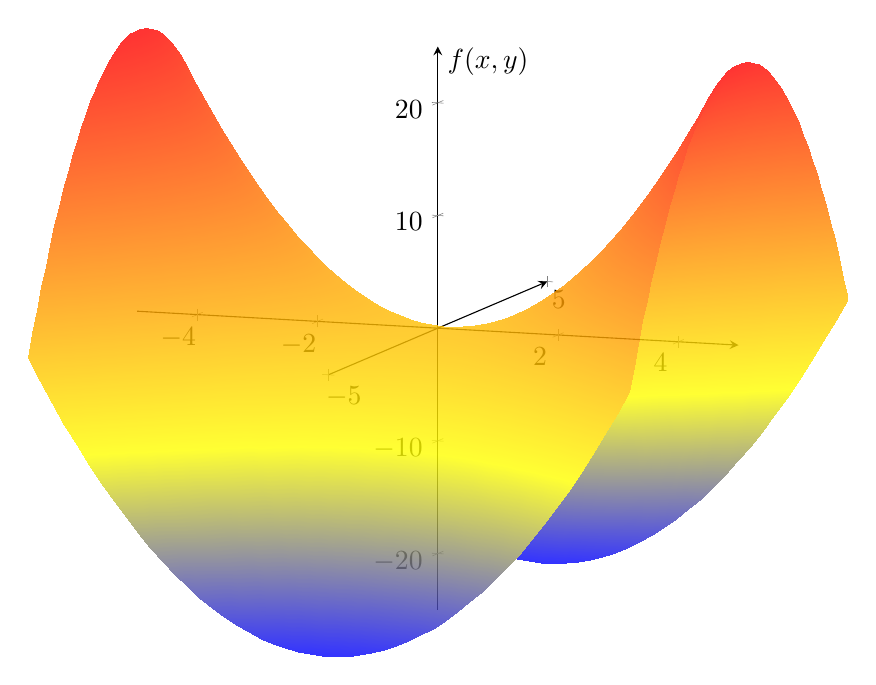
\begin{tikzpicture}
    % Definisco lo stile dei vettori
    \tikzset{vector/.style={-stealth, thick, color=black}}

    % Parametri per il punto di contatto
    \def\xo{1}
    \def\yo{2}
    \def\zo{5} % Calcola z0 = f(x0, y0)

    % Derivate parziali della funzione f(x, y) = x^2 + y^2 nel punto (x0, y0)
    \def\fx{2*\xo} % = 2
    \def\fy{2*\yo} % = 4

    % Disegno la superficie
    \begin{axis}[
        width=12cm,
        view={20}{10}, % Angolazione impostata
        axis lines=middle,
        zlabel={$f(x,y)$},
        clip=false,
        domain=-5:5,
        y domain=-5:5,
        samples=50,
        z buffer=sort
    ]
    % Grafico della superficie con colore visibile
    \addplot3[surf, opacity=0.8, shader=interp]
        {x^2 - y^2}; % Superficie f(x, y) = x^2 + y^2
    \end{axis}
\end{tikzpicture}
\label{fig:punto_sella}
\caption{Grafico della funzione $f(x, y) = x^2 - y^2$: come è possibile vedere il punto $(0, 0)$ non è né un punto di minimo locale né un punto di massimo locale: si tratta di un \emph{punto di sella}}
\end{figure}
Enunciamo il seguente criterio
\begin{theorem}[condizione sufficiente per il massimo/minimo locale]
Sia $f:\Omega \to \mathbb{R}, f \in C^2 (\Omega)$ con $\Omega \subseteq \mathbb{R}^n$ aperto e sia $x_0 \in \Omega$ un punto critico di f ($\nabla f(x_0) = 0$). Se $Hf(x_0)$ è definita positiva, allora $x_0 \in \Omega$ è un punto di minimo locale per $f$; altrimenti se $Hf(x_0)$ è definita negativa, allora $x_0$ è un punto di massimo locale per $f$.
\end{theorem}
\begin{proof} Senza perdita di generalità, facciamo la dimostrazione supponendo che $Hf(x_0)$ sia definita positiva (il caso della matrice hessiana definita negativa è simile). 
Per il teorema della formula di Taylor~~\ref{thm:form_taylor} abbiamo che
$$
f(x) = f(x_0) + \frac{1}{2} \innerprod{Hf(x_0)(x-x_0)}{x-x_0} + o(|x-x_0|^2) \text{ per } x \to x_0
$$
Consideriamo adesso $\lambda = \min\limits_{v \in \mathbb{S}^{n-1}} \innerprod{Hf(x_0)v}{v} > 0$ per l'ipotesi di positività di $Hf(x_0)$. Allora sappiamo che $\exists \delta > 0$ tale che $B(x_0, \delta) \subseteq \Omega$ e $|o(|x-x_0|^2)| < \frac{\lambda}{2}|x-x_0|^2$ per $0 < |x-x_0| < \delta$, dunque
$$
o(|x-x_0|^2) \geq -|o(|x-x_0|^2)| \geq -\frac{\lambda}{2}|x-x_0|^2
$$
dunque $\forall x \in B(x_0, \delta) \setminus \{ x_0 \}$
\begin{align*}
&f(x) = f(x_0) + \frac{1}{2}\innerprod{Hf(x_0)(x-x_0)}{(x-x_0)} + o(|x-x_0|^2) = \\
&=f(x_0) + \frac{1}{2} \innerprod{Hf(x_0)\frac{x-x_0}{|x-x_0|}}{\frac{x-x_0}{|x-x_0|}}|x-x_0|^2 + o(|x-x_0|^2) \geq \\
&\geq f(x_0) + \frac{\lambda}{2}|x-x_0|^2 - \frac{\lambda}{2}|x-x_0|^2 = f(x_0) \implies f(x) \geq f(x_0)
\end{align*}
questo conclude la dimostrazione.
\end{proof}
Adesso vogliamo trovare un criterio con cui stabilire quando i punti critici sono di sella. Anche in questo caso tramite il comportamento al \emph{secondo ordine} della funzione (ovvero dalla matrice hessiana) possiamo stabilirlo tramite il seguente teorema
\begin{theorem}[dei punti di sella]
Sia $f \in C^2(\Omega), x_0 \in \Omega, \nabla f(x_0) = 0$, $\det{Hf(x_0)} \neq 0$ e $Hf(x_0)$ non è definita positiva e non è definita negativa
$$
\implies x_0 \text{ non è né di massimo locale né di minimo locale}
$$
\end{theorem}
\begin{proof}
$$
Hf(x_0)=A=A^T=C^T \Lambda C
$$
dove $\Lambda = \begin{pmatrix} \lambda_1 & 0 & \ldots & 0 \\
0 & \lambda_2 & \ldots & 0 \\
0 & 0 & \ddots & 0 \\ 0 & \ldots & \ldots & \lambda_n \end{pmatrix}$ e $\lambda_1, \ldots, \lambda_n$ autovalori reali. Osserviamo che
$$
\innerprod{Ax}{x} = \innerprod{C^T \Lambda Cx}{Cx} = \innerprod{\Lambda Cx}{Cx} =  \innerprod{\Lambda Cx}{Cx} \stackrel{y=Cx}{=} \innerprod{\Lambda y}{y} = \sum_{j=1}^n \lambda_j y_j^2
$$
Osserviamo che, grazie al teorema spettrale, $\forall j \in \{1, \ldots, n \} \, \exists v_j \in \mathbb{S}^{n-1} : e_j = Cv_j$ dove $v_j$ è il $j-$esimo autovettore
$$
Av_j = C^{-1} \Lambda Cv_j = C^{-1} \Lambda e_j = C^{-1} (\lambda_j e_j) = \lambda (C^{-1} e_j) = \lambda_j v_j
$$
dunque
$$
\innerprod{Hf(x_0)v_j}{v_j} = \lambda_j
$$
Dalla formula di Taylor concludiamo che
$$
f(x_0 + tv_j) = f(x_0) + \frac{1}{2} \innerprod{Hf(x_0)tv_j}{tv_j} + o(|tv_j|^2) = f(x_0) + t^2 \left( \frac{\lambda_j}{2} + o(1) \right)
$$
poiché $Hf(x_0)$ non è né definita positiva né definita negativa avremo che $\lambda_j > 0$ e $\lambda_j < 0$ dunque la precedente uguaglianza, unita al ragionamento compiuto nella dimostrazione del teorema precedente portano alla tesi.
\end{proof}
\begin{remark}
In questa dimostrazione comprendiamo come mai si chiamino \emph{punti di sella}: nel caso $n=2$ (ovvero in due dimensioni) con la seguente matrice hessiana
$$
Hf(x_0) = \begin{pmatrix}
2 & 0 \\
0 & -2
\end{pmatrix}
$$
vuol dire che la funzione, lungo una direzione, assume un massimo locale in quel punto e nell'altra un minimo. La funzione $f(x,y)=x^2-y^2$ (Figura~\ref{fig:punto_sella}) nel punto $(0,0)$ lungo la direzione $x$ ha un punto minimo (basti osservare la restrizione della funzione a $y=0$, per cui otteniamo $f(x, 0)=x^2$) e un punto di massimo (basti osservare la restrizione della funzione a $x=0$, per cui otteniamo $f(0, y) = -y^2$). Il motivo della terminologia \emph{punto di sella} deriva proprio del fatto che in due dimensione assume proprio la forma di una sella.
\end{remark}
Il problema è capire come si comporta nei punti per cui è presente un autovalore nullo: purtroppo, quando l'hessiana è semi-definita abbiamo bisogno di procedere tramite dei ragionamenti più sofisticati che dipendono da caso a caso.